\chapter{The Schwarzschild Solution}
As described in the previous chapter, the theory of general relativity has made a number of strikingly successful predictions concerning the spacetime structure of our universe. However, cosmological observations presently are not good enough to provide stringent quantitative tests of general relativity. Such quantitative tests are provided by the gravitational fields occurring in our solar system, where precise measurements can be made. Thus, it is of great interest to determine the solution of Einstein's equation corresponding to the exterior gravitational feld of a static, spherically symmetric body (such as are our Sun and many other bodies, to an excellent approximation). This problem was solved by Karl Schwarzschild (1916a), only a few months after Einstein published his vacuum field equations. The Schwarzschild solution without question remains one of the most important known exact solutions of Einstein's equation.

As was previously discussed in section 4.4a, in the slow motion, weak field limit, the predicitons of general relativity reduce to those of Newtonian theory. However, the Schwarzschild solution, which describes the exact exterior field of a spherical body, predicts tiny departures from Newtonian theory for the motion of planets in our solar system, and, in addition, predicts the ``bending of light'', the gravitational redshift of light, and ``time delay'' effects. These four predictions have been accurately confirmed by precise measurements. Indeed, except for the binary pulsan measurements (see the end of chapter 4), the predictions of the Schwarzschild solution in the weak field regime of our solar system are the only predictions of general relativity to have been tested in a quantitatively precise manner.

But the Schwarzschild solution has provided us with a great deal more than the ability to predict tiny effects occurring in our solar system. As will be discussed further in section 6.2, sufficientlymassivebodiesareunabletosupportthemselves against complete gravitational collapse. After the collapse of a spherical body has occurred, the entire spacetime geometry will be described by the Schwarzschild solution, and thus the Schwarzschild solution tells us a great deal about the strong field behavior of general relativity. As will be seen in section 6.4, the vacuum Schwarzschild solution describing the end-product of gravitational collapse contains a spacetime singularity which is hidden within a black hole.

We shall derive the Schwarzschild solution in section 6.1, using the tetrad method of section 3.4b. In section 6.2 we consider the interior matter sources of the exterion vacuum Schwarzschild solution and thereby derive the relativistic equations of stellar structure. The timelike and null geodesics of the Schwarzschild metric are studied in section 6.3 and are used there to make predictions for the four tests of general relativity: the gravitational redshift, the precession of Mercury's orbit, the bending of light, and the ``time delay'' of light. Finally, in section 6.4 we examine the strong field regime of the vacuum Schwarzschild solution.

% \section{Derivation of the Schwarzschild Solution}
% \section{Interior Solutions}
% \section{Geodesics of Schwarzschild: Gravitational Redshift, Perihelion Precession, Bending of Light, and Time Delay}
% \section{The Kruskal Extension}

% \includepdf[pages=53-59]{document}